\documentclass{article}

\usepackage{fullpage}
\usepackage{parskip}
\usepackage{setspace}
\usepackage{mathtools}
\usepackage{tikz}
\usetikzlibrary{arrows}
\usetikzlibrary{decorations.markings}
\usetikzlibrary{calc}
\usepackage{standalone}
\usepackage{float}
\usepackage{caption}
\usepackage{subcaption}
\usepackage{amsmath}
\usepackage{amsfonts}
\usepackage{amsthm}
\usepackage[ruled]{algorithm2e}

\newtheorem{definition}{Definition}
\newtheorem{theorem}{Theorem}
\newtheorem{lemma}{Lemma}

\title{Detecting Deadlock in Discrete Event Simulations of Queueing Networks}
\author{Geraint Palmer}
\date{}

\begin{document}
\onehalfspacing

\maketitle

This section will define and discuss the properties and detection of deadlock in queueing networks.
Throughout the section, when discussing queueing networks, it is assumed that
the queueing network is open and connected.
Open queueing networks are those networks that have at least one node to which customers arrive from the exterior, and and least one node from which customers leave to the exterior.

\section{Deadlock}

\begin{definition}
    When a simulation is in a situation where at least one service station,
    despite having arrivals, ceases to finish any more services
    due to recursive upstream blocking the system is said to be in deadlock.
\end{definition}

Deadlock can be experienced in any open queueing network that experiences
blocking, with at least once cycle containing all service stations with
resticted queueing capacity.

Deadlock occurs when a customer finishes service at node $i$ and is blocked from transitioning to node $j$; however the individuals in node $j$ are all blocked, directly or indirectly, by the blocked individual in node $i$.
That is, deadlock occurs if every individual blocking individual $X$, directly or indirectly, are also blocked.

In Figure~\ref{fig:2in_deadlock} a simple two node queueing network is shown in a deadlocked state.
Customer occupying server $A_1$ has finished service at node $A$, but remains there as there is not
enough queueing space at node $B$ to accept them.
We say the customer at server $A_1$ is blocked by the customer at server $B_1$, as he is waiting for that customer to be released.
Similarly, the customer occupying server $B_1$ has finished service at node $B$, but remains there as there is not enough queueing space at node $A$, and so the customer at server $B_1$ is blocked by the customer at server $A_1$.

When there are multiple servers, individuals become blocked by all customers in
service at the destination service station.
Figure~\ref{fig:inout_deadlock_in} shows two nodes in deadlock, the customer occupying server $A_1$ is blocked by customers at both $B_1$ and $B_2$, who are both blocked by the customer at $A_1$.
However in \ref{fig:inout_deadlock_out}, customer at $A_1$ is blocked by customers at both $B_1$ and $B_2$, but the customer at $B_2$ isn't blocked, and so there is no deadlock.

\begin{figure}[H]
  \begin{center}
  \includestandalone[width=0.5\textwidth]{images/2nodesindeadlock}
  \caption{Two nodes in deadlock.}
  \label{fig:2in_deadlock}
  \end{center}
\end{figure}

\begin{figure}[H]
\begin{subfigure}[b]{0.5\textwidth}
  \includestandalone[width=0.9\textwidth]{images/2nodesindeadlockmulti}
  \caption{Two nodes in deadlock.}
  \label{fig:inout_deadlock_in}
\end{subfigure}
\begin{subfigure}[b]{0.5\textwidth}
  \includestandalone[width=0.9\textwidth]{images/2nodesnotdeadlocked}
  \caption{Two nodes not deadlocked}
  \label{fig:inout_deadlock_out}
\end{subfigure}
\caption{Two nodes: a) in deadlock and b) not in deadlock.}
\label{fig:inout_deadlock}
\end{figure}

Note that the whole queueing network need not be deadlocked, only a part of it.
If one section of the network is in deadlock, then the system is deadlocked, even though customers may still be able to have services and transitions in other areas of the network.
An example is shown in Figure~\ref{fig:trans}.
This idea is expanded on in the next section.

\section{Types of Deadlock}
The previous section introduced the idea that parts of a queueing network can be in a deadlocked state, although other parts will continue to flow.
The different configurations of which nodes experience deadlock can be thought
of as different types of deadlock.
The amount of different types of deadlock that a queueing network can experience
is equal to the number of directed cycles in in the queueing network's routing
matrix. % This paragraph will change and will need more discussion of last
%sentence (images etc...)

For connected queueing networks, these deadlocks can be classified into transient deadlocked states and the absorbing deadlocked state.\\


\begin{definition}
    A transient deadlock state is when there are still some changes of state
    whilst a subgraph of the queueing network is itself in deadlock.\\
\end{definition}

\begin{definition}
    The absorbing deadlock state is when all subgraphs of the
    queueing network are in deadlock.\\
\end{definition}

Figure~\ref{fig:transabsorb} shows a three nodes network in a transient deadlocked state, and an absorbing deadlocked state.
In Figure~\ref{fig:trans} the occupants of servers $B_1$ and $B_2$ are blocked from entering node $A$; and the occipant of server $A_1$ is blocked from entering node $B$, and so these two nodes are in deadlock.
However, node $C$ can continue with regular services, until the occupants of every server of $C$ attempt to join a deadlocked node.
At which point, the whole system is deadlocked, and so has reached absorbing deadlock, show in Figure~\ref{fig:absorb}.

\begin{figure}[H]
\begin{subfigure}[b]{0.5\textwidth}
  \includestandalone[width=0.9\textwidth]{images/transientdeadlock}
  \caption{Transient deadlock.}
  \label{fig:trans}
\end{subfigure}
\begin{subfigure}[b]{0.5\textwidth}
  \includestandalone[width=0.9\textwidth]{images/absorbingdeadlock}
  \caption{Absorbing deadlock.}
  \label{fig:absorb}
\end{subfigure}
\caption{Types of deadlock: a) transient and b) absorbing.}
\label{fig:transabsorb}
\end{figure}

For a queueing network $Q$ with $N$ service stations, the absorbing deadlocked state corresponds to $(i_1=-1,...,i_N=-1)$, the state where all service stations experience deadlock.
It should be clear that if the queueing network is connected, then there is a non-zero probability that once one part of the network is in deadlock, the whole system will fall into a deadlocked state, simply by the individuals in the non-deadlocked nodes attempting to transition into a deadlocked node.
That is, once $Q$ falls into one of the transient deadlocked states, it will eventually transition, either directly or through other transient deadlocked states, into the absorbing deadlocked state.

If the routing matrix of $Q$ is complete, that is there is a possible route from every service station to every other service station, then there are $\sum_{i=1}^N \binom{N}{i}$ possible deadlock types.

\section{Literature Review}

Most of the literature on blocking either does not consider networks with feedback loops, ignores the possibility of deadlock, or conveniently assumes the networks are
deadlock-free.
For closed networks of $K$ customers with only one class of customer, \cite{kunduakyildiz89} proves the following condition to ensures no deadlock: for each minimum cycle $C$, $K < \sum_{j\in C} B_j$, the total number of customers cannot exceed the total queueing capacity of each minimum subcycle of the network.
The paper also presents algorithms for finding the minimum queueing space required to ensure deadlock never occurs, for closed cactus networks, where no two cycles have more than one node in common.
This result is extended to multiple classes of customer in \cite{liebeherrakyildiz95}, with more restrictions such as single servers and each class having the same service time distribution.
Here a integer linear program is formulated to find the minimum queueing space assignment that prevents deadlock.
The literature does not discuss deadlock properties in open restricted queueing networks.

General deadlock situations that are not specific to queueing networks are discussed in \cite{coffmanelphick71}.
Conditions for this type of deadlock, also referred to as deadly embraces, to potentially occur are given:
\begin{itemize}
  \item Mutual exclusion: Tasks have exclusive control over resources.
  \item Wait for: Tasks do not release resources while waiting for other resources.
  \item No preemption: Resources cannot be removed until they have been used to completion.
  \item Circular wait: A circular chain of tasks exists, where each task requests a resource from another task in the chain.
\end{itemize}
Dynamic state-graphs are defined, with resources as vertices and requests as edges.
For scenarios where there is only one type of each resource, deadlock arises if and only if the state-graph contains a cylce.

In \cite{choetal95} the vertices and edges of the state graph are given labels in relation to a reference node.
Using these labels \textit{simple bounded circuits} are defined whose existance within the state graph is sufficient to detect deadlock.


\section{Definitions}

\begin{tabular}{ p{5cm} p{10cm} }
  $\left| V(D) \right|$        & The order of the directed graph $D$ is its number of vertices. \\
  Weakly connected component   & A weakly connected component of a digraph containing $X$ is the set of all nodes that can be reached from $X$ if we ignore the direction of the edges. \\
  Direct successor             & If a directed graph contains an edge from $X_i$ to $X_j$ , then we say that $X_j$ is a direct successor of $X_i$. \\
  Ancestors                    & If a directed graph contains a path from $X_i$ to $X_j$ , then we say that $X_i$ is an ancestor of $X_j$. \\
  Descendants                  & If a directed graph contains a path from $X_i$ to $X_j$ , then we say that $X_j$ is a descendant of $X_i$. \\
  $\text{deg}^{\text{out}}(X)$ & The out-degree of $X$ is the number of outgoing edges emanating from that vertex. \\
  Subgraph                     & A subgraph $H$ of a graph $G$ is a graph whose vertices are a subset of the vertex set of $G$, and whose edges are a subset of the edge set of $G$. \\
  Sink vertex                  & A sink vertex is a vertex in a directed graph that has out-degree of zero.\\
  Knot                         & In a directed graph, a knot is a set of vertices with out-edges such that while traversing the directed edges of that directed graph, once a vertex in the knot is reached, you cannot rech any vertex that is not in the knot.\\
\end{tabular}


\section{State Digraph}

Presented is a method of detecting when deadlock occurs in an open queueing network $Q$ with $N$ nodes, using a dynamic directed graph, the state graph.

Let the number of servers in node $i$ be denoted by $c_i$.
Define $D(t)=(V(t), E(t))$ as the state graph of $Q$ at time $t$.

The vertices at time \(t\), \(V(t)\) correspond to servers in the
queueing system.
Thus, $\left| V\left(D\left(t\right)\right) \right| = \sum_{i=1}^N c_i$ for all $t \geq 0$.

The edges at time \(t\), \(E(t)\) correspond to a blocking relationship.
There is a directed edge at time \(t\) from vertex \(X_a\in V(t)\) to vertex \(X_b\in
V(t)\) if and only if an individual occupying the server corresponding to vertex
\(X_a\) is being blocked by an individual occupying the server corresponding to
vertex \(X_b\).

The state graph $D(t)$ can be partitioned into $N$ service-station subgraphs,
$D(t)=\bigcup_{i=1}^N d_i(t)$, where the vertices of $d_i(t)$ represent the servers of node $i$.
The vertex set of each subgraph is static over time, however their edge sets may
change.

The state graph is dynamically built up as follows.
When an individual finishes service at node $i$, and this individual's next destination is node $j$, but there is not enough queueing capacity for $j$ to accept that individual, then that individual remains at node $i$ and becomes blocked.
At this point $c_j$ directed edges between this individual's server and the vertices of $d_j(t)$ are created in $D(t)$.

When an individual is released and another customer who wasn't blocked occupies their server, that servers out-edges are removed.
When an individual is released and another customer who was previously blocked occupies their server, that server's out-edges are removed along with the in-edge from the server who that previously blocked customer occupied.
When an individual is released and there isn't another customer to occupy that server, then all edges incident to that server are removed.

This general process of building up the state graph as the queueing network is simulated will now be shown.
Customers are labelled $(i, j, k)$ where $i$ denotes the server that customer is occupying, $j$ denotes that individuals i.d. number, and $k$ denotes the service station that customer is waiting to enter.
As an example, a customer labelled $(A_2, 10, C)$ would have an i.d. number of 2, is occupying server $A_2$ and is currently waiting to join node $C$.
If a customer isn't occupying a server the notation $\emptyset$ is used.
Similarly for customers occupying a server and still in service, their next destination is yet undecided, so $\emptyset$ is used.

The simulation starts with full queues, and every server occupied by a customer in service. This is shown in Figure~\ref{fig:general_buildup_1}.

\begin{figure}[H]
  \begin{tabular}{ c c c }
      \includestandalone[width=0.62\textwidth]{images/examplenetwork2_scen1_step1} & \hspace{0.1\textwidth} &
      \includestandalone[width=0.2\textwidth]{images/exampledigraph_scen1_step1} \\
  \end{tabular}
  \caption{}
  \label{fig:general_buildup_1}
\end{figure}

Customer 13 finishes service, and is blocked from entering node $A$. Figure~\ref{fig:general_buildup_2}.

\begin{figure}[H]
  \begin{tabular}{ c c c }
      \includestandalone[width=0.62\textwidth]{images/examplenetwork2_scen1_step2} & \hspace{0.1\textwidth} &
      \includestandalone[width=0.2\textwidth]{images/exampledigraph_scen1_step2} \\
  \end{tabular}
  \caption{}
  \label{fig:general_buildup_2}
\end{figure}

Then customer 4 finishes service and is blocked from entering node $B$. Figure~\ref{fig:general_buildup_3}.

\begin{figure}[H]
  \begin{tabular}{ c c c }
      \includestandalone[width=0.62\textwidth]{images/examplenetwork2_scen1_step3} & \hspace{0.1\textwidth} &
      \includestandalone[width=0.2\textwidth]{images/exampledigraph_scen1_step3} \\
  \end{tabular}
  \caption{}
  \label{fig:general_buildup_3}
\end{figure}

Then customer 9 finishes service and is blocked from entering node $A$. Figure~\ref{fig:general_buildup_4}.

\begin{figure}[H]
  \begin{tabular}{ c c c }
      \includestandalone[width=0.62\textwidth]{images/examplenetwork2_scen1_step4} & \hspace{0.1\textwidth} &
      \includestandalone[width=0.2\textwidth]{images/exampledigraph_scen1_step4} \\
  \end{tabular}
  \caption{}
  \label{fig:general_buildup_4}
\end{figure}

Finally, in Figure~\ref{fig:general_buildup_5} customer 5 finishes service and wants to reenter the queue for node $A$ but is blocked.
A deadlock situation arises as customer 5 is waiting for customer 4 to move, who is waiting for customer 9 to move, who is waiting for either customer 4 or 5 to move.

\begin{figure}[H]
  \begin{tabular}{ c c c }
      \includestandalone[width=0.62\textwidth]{images/examplenetwork2_scen1_step5} & \hspace{0.1\textwidth} &
      \includestandalone[width=0.2\textwidth]{images/exampledigraph_scen1_step5} \\
  \end{tabular}
  \caption{}
  \label{fig:general_buildup_5}
\end{figure}

The rules on how edges are removed from the state graph will now be shown.
For illustrative purposes the queueing network here is a different queueing network than discussed above.

Here the simulation begins with four customers occupying servers; those at node $A$ blocked to node $B$, the customer at node $C$ blocked to node $A$, and the customer at node $B$ still in service.
This is shown in Figure~\ref{fig:general_builddown_1}.

\begin{figure}[H]
  \begin{center}
    \begin{tabular}{ c c c }
      \includestandalone[width=0.62\textwidth]{images/examplenetwork2_scen2_step1} & \hspace{0.1\textwidth} &
      \includestandalone[width=0.2\textwidth]{images/exampledigraph_scen2_step1} \\
  \end{tabular}
  \end{center}
  \caption{}
  \label{fig:general_builddown_1}
\end{figure}

Customer 6 finishes service and immediately joins service at node $C$. Figure~\ref{fig:general_builddown_2}.

\begin{figure}[H]
  \begin{center}
    \begin{tabular}{ c c c }
      \includestandalone[width=0.62\textwidth]{images/examplenetwork2_scen2_step2} & \hspace{0.1\textwidth} &
      \includestandalone[width=0.2\textwidth]{images/exampledigraph_scen2_step2} \\
  \end{tabular}
  \end{center}
  \caption{}
  \label{fig:general_builddown_2}
\end{figure}

Now there is room for customer 4 to move into service at node $B$. Figure~\ref{fig:general_builddown_3}.
Notice that the edge $A_2 \longrightarrow B_1$ remains in the state graph, as customer 5 is still blocked by that server.

\begin{figure}[H]
  \begin{center}
    \begin{tabular}{ c c c }
      \includestandalone[width=0.62\textwidth]{images/examplenetwork2_scen2_step3} & \hspace{0.1\textwidth} &
      \includestandalone[width=0.2\textwidth]{images/exampledigraph_scen2_step3} \\
  \end{tabular}
  \end{center}
  \caption{}
  \label{fig:general_builddown_3}
\end{figure}

The customers queueing at node $A$ move along the queue, with customer 3 begining service.
This leaves enough room for customer 7 to join the back of the queue at $A$. Figure~\ref{fig:general_builddown_4}.

\begin{figure}[H]
  \begin{center}
    \begin{tabular}{ c c c }
      \includestandalone[width=0.62\textwidth]{images/examplenetwork2_scen2_step4} & \hspace{0.1\textwidth} &
      \includestandalone[width=0.2\textwidth]{images/exampledigraph_scen2_step4} \\
  \end{tabular}
  \end{center}
  \caption{}
  \label{fig:general_builddown_4}
\end{figure}

\subsubsection*{Observations}

Consider one weakly connected component $G(t)$ of $D(t)$.
Consider the node $X_a \in G(t)$. If $X_a$ is unoccupied, then $X_a$ has no incident edges.
Consider the case when $X_a$ is occupied by individual $a$, whose next destination is node $j$.
Then $X_a$'s direct successors are the servers occupied by individuals who are blocked or in service at node $j$.
We can interpret all $X_a$'s decendents as the servers whose occupants are directly or indirectly blocking $a$, and we can interpret all $X_a$'s ancestors as those servers whose individuals who are being blocked directly or indirectly by $a$.

Note that the only possibilities for $\text{deg}^{\text{out}}(X_a)$ are being 0 or $c_j$.
If $\text{deg}^{\text{out}}(X_a) = c_j$ then $a$ is blocked by all its direct successors.
The only other situation is that $a$ is not blocked, and $X_a \in G(t)$ because $a$ is in service at $X_a$ and blocking other individuals, in which case $\text{deg}^{\text{out}}(X_a) = 0$.

It is clear that if all of $X_a$'s descendents are occupied by blocked individuals, then the system is deadlocked at time $t$.
We also know that by definition all of $X_a$'s ancestors are occupied by blocked individuals.

Also note that if a service-station subgraph $d_i(t)$ contains edges, then there is an individual in $X_a \in d_i(t)$ that is being blocked by himself.
This does not necassarily mean there is deadlock.


\section{Results on the State Digraph}

\begin{theorem}
A deadlocked state arises at time $t$ if and only if $D(t)$ contains a knot.
\end{theorem}

\begin{proof}
Consider one weakly connected component $G(t)$ of $D(t)$ at time $t$.
All vertices of $G(t)$ are either decendents of another vertex and so are occupied by an individual who is blocking someone; or are ancestors of another vertex, and so are occupied by someone who is blocked.

Assume that $G(t)$ contains a vertex $X$ such that $\text{deg}^{\text{out}}(X) = 0$, and there is a path from every other non-sink vertix to $X$.
This imples that $X$'s occupant is not blocked and is a descendent of another vertrex.
Therefore $Q$ is not deadlocked as there does not exist a vertex whose descendents are all blocked.

Now assume that we have deadlock.
For a vertex $X$ who is deadlocked, all decendents of $X$ are are occupied by individuals who are blocked, and so must have out-degrees greater than 0.
And so there is no path from $X$ to a vertex with out-degree of 0.
\end{proof}


\begin{lemma}
For a queueing network with two nodes or less, a deadlocked state arises if and only if there exists a weakly connected component without a sink node.
\end{lemma}

\begin{proof}
Consider a one node queueing network $Q_1$.

If there is deadlock, then all servers are occupied by blocked individuals, and so all servers have an out-edge.

Consider a two node queueing network $Q_2$.

If both nodes are involved in the deadlock, so there is a customer in node 1 blocked from entering node 2, and a customer from node 2 blocked from entering node 1, then all servers in node 1 and node 2 in $D(t)$ will have out edges as they are occupied by a blocked individual.
The servers of node 1 and 2 consist of the entirety of $D(t)$, and so there is no sink nodes.

Now consider the case when only one node is involved in the deadlock.
Without loss of generality, let's say that node 1 is in deadlock with itself, then the servers of node 1 have out-edges.
For the servers of node 2 to be part of that weakly conneced component, there either needs to be an edge from a server in node 1 to a server in node 2, or and edge from a server in node 2 to a server in node 1.
An edge from a server in node 1 to a server in node 2 implies that a customer from node 1 is blocked from entering node 2, and so node 1 is not in deadlock with itself.
An edge from a server in node 2 to a server in node 1 implies that a customer in node 2 is blocked from entering node 1.
In this case the server in node 2 has an out-edge, and so there is still no sink.

For the case of a queueing network with more than two nodes, the following counter-example proves the claim:

Begin with all servers occupied by customers in service.
The customer at server $B_1$ is blocked from entering node $A$.
Then the customer at server $C_1$ is blocked from entering node $B$.
Then the customer at server $A_1$ is blocked from entering node $A$.
The resulting state digraph in Figure~\ref{fig:counter_example} has a weakly connected component with a sink.
\end{proof}

\begin{figure}
\begin{center}
\includestandalone[width=0.3\textwidth]{images/counter_example_digraph}
\end{center}
\caption{A Counter-Example State Digraph.}
\label{fig:counter_example}
\end{figure}

\begin{lemma}
An absorbing deadlocked state arises at time $t$ if $D(t)$ doesn't contain a sink vertex.
\end{lemma}

\begin{proof}
A vertex with out-degree greater than zero represents an occupied server whose occupant has finished service and is blocked.
If all vertices have out-degree greater than zero, then all servers are occupied by blocked individuals.
A release at vertex $X_a$ can only be triggered by one of $X_a$'s descendents finishing service.
As all servers are occupied by blocked individuals, no server can finish service, and so no server can release their occupant, implying an absorbing deadlocked state.
\end{proof}

\section{Finding Knots}

By definition knots are strongly connected subgraphs where every member's descendants belong to that subgraph.

Using the Python package NetworkX, finding strongly connected components, and finding a vertex's decendants are built-in methods.
The following algoithm, taken from the NetworkX developer zone ticket \#663, is sufficient to identify knots in a directed graph.

\begin{algorithm}[H]
    \DontPrintSemicolon
    Find the strongly connected subgraphs of $D(t)$\;
    \For{strongly connected subgraph $SCS$ in list of strongly connected subgraphs of $D(t)$}{
      \For{vertex $v$ in $SCS$}{
        \If{number of $v$'s decendants $>$ number of vertices in $SCS$}{
          Add $SCS$ to list of knots\;
          break\;
          }\;
        }\;
      }\;
\end{algorithm}



\section{Markov Chain Model}

It is interesting to build an analytical model of the system's behaviour to deadlock.
As a Markov chain model, the deadlocking state is an absorbing state, and so any queueing network that can experience deadlock is guaranteed to experience deadlock.

We can however find the expected time until deadlock is reached.
It is shown in \cite{stewart09} that for a discrete transition matrix of the form $P = \bigl(\begin{smallmatrix} T & U\\ 0 & V \end{smallmatrix} \bigr)$ then the expected number of time steps until absorbtion starting from state $i$ is the $i\text{th}$ element of the vector
\begin{equation}
  (I - T)^{-1}e
\end{equation}
where $e$ is a vector of 1s.
% this.

Another interesting analytical measure to find is the median time to deadlock.

\subsection{One Node Network}
Consider the one node network with feedback loop shown in Figure~\ref{fig:queueingnetwork_1node}.
There is room for $n$ customers to queue at any one time, customers arrive at a rate of $\Lambda$ and served at a rate $\mu$.
Once a customer has finished service he rejoins the queue with probability $r_{11}$, and so exits the system with probability $1 - r_{11}$.

\begin{figure}[H]
  \includestandalone[width=\textwidth]{images/1nodeexample}
  \caption{A one node queueing network.}
  \label{fig:queueingnetwork_1node}
\end{figure}

State space:
        \[S = \{i\in\mathbb{N}| 0 \leq i \leq n + 1
        \}\cup\{-1\}\]
where \(i\) denotes number of individuals in service or waiting.

If we define $\delta = i_2 - i_1$ for all $i_k \in S | i_k \geq 0$, then the transitions are given by:

\begin{equation}
  q_{i_1, i_2} = \left\{
  \begin{matrix*}[ r ]
    \left. \begin{matrix*}[ r ]
      0 & \text{if } i = n + 1 \\
      \Lambda & \text{otherwise}
    \end{matrix*} \right\} & \text{if } \delta = 1 \\
    (1 - r_{11})\mu & \text{if } \delta = -1 \\
    0 & \text{otherwise}
  \end{matrix*} \right.
\end{equation}

\begin{equation}
  q_{i, -1} = \left\{
  \begin{matrix*}[ r ]
    r_{11}\mu & \text{if } i = n + 1) \\
    0 & \text{otherwise}
  \end{matrix*}
  \right.
\end{equation}

and

\begin{equation}
  q_{-1, i} = 0
\end{equation}

The Markov chain is shown in Figure~\ref{fig:1nodeMC}.

\begin{figure}[H]
    \includestandalone[width=\textwidth]{images/markov_chain_1node}
    \caption{Markov chain of the one node system.}
    \label{fig:1nodeMC}
\end{figure}

Figure~\ref{fig:timestodeadlock} shows the effect of varying the parameters of the queueing network on times to deadlock.
We can see that increasing the arrival rate $\Lambda$ and the transition probability $r_{11}$ results in reaching deadlock faster.
This is intuitive as increasing these parameters results in the first node's queue filling up quicker.
Increasing the queueing capacity $n$ results in reaching deadlock slower.
Again this are intuitive, as increasing the queueing capacity allows more customers in the system before becoming deadlock.


\begin{figure}
\begin{subfigure}[b]{0.5\textwidth}
  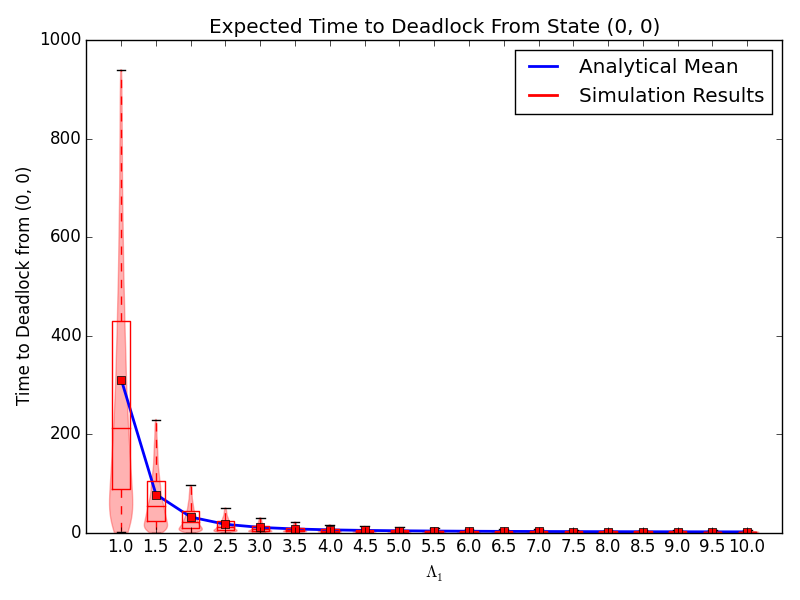
\includegraphics[width=\textwidth]{images/varyL}
  \caption{Varying $\Lambda$}
  \label{fig:timestodeadlock_L}
\end{subfigure}
\begin{subfigure}[b]{0.5\textwidth}
  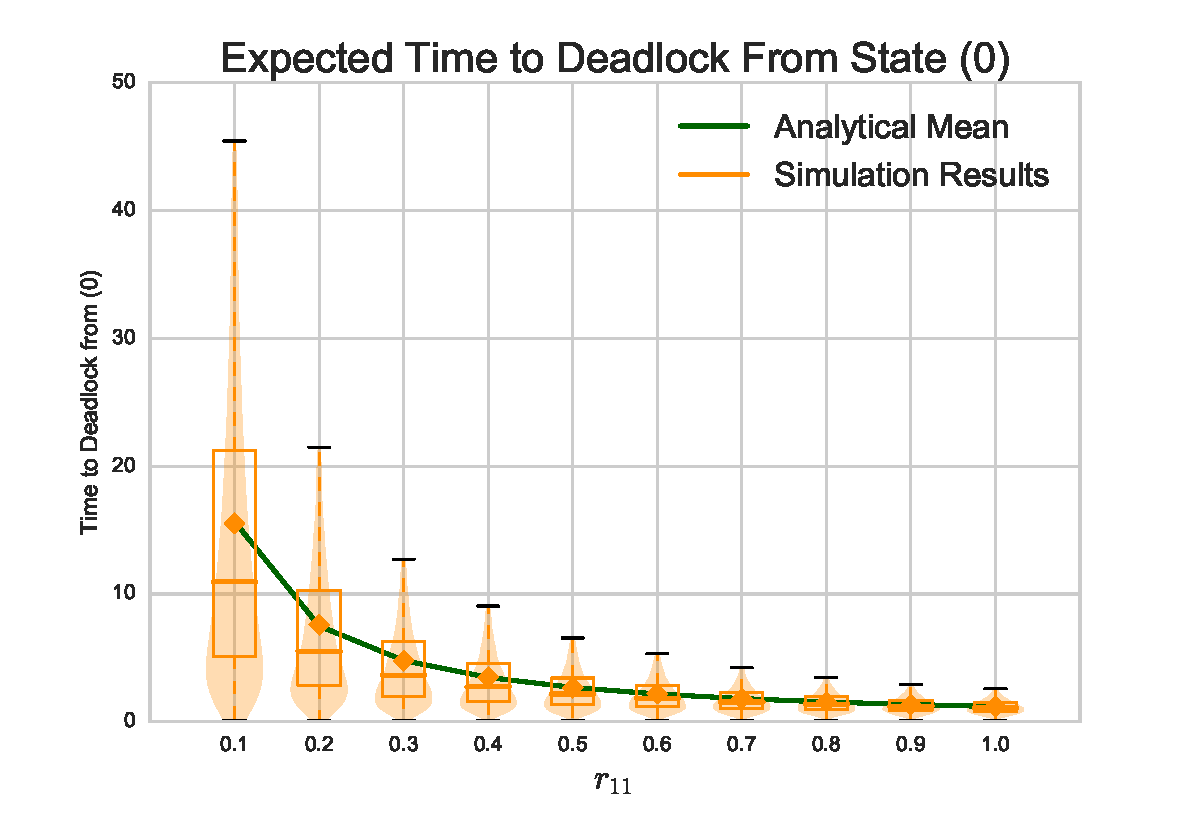
\includegraphics[width=\textwidth]{images/varyr11}
  \caption{Varying $r_{11}$}
  \label{fig:timestodeadlock_r11}
\end{subfigure}
\begin{subfigure}[b]{0.5\textwidth}
  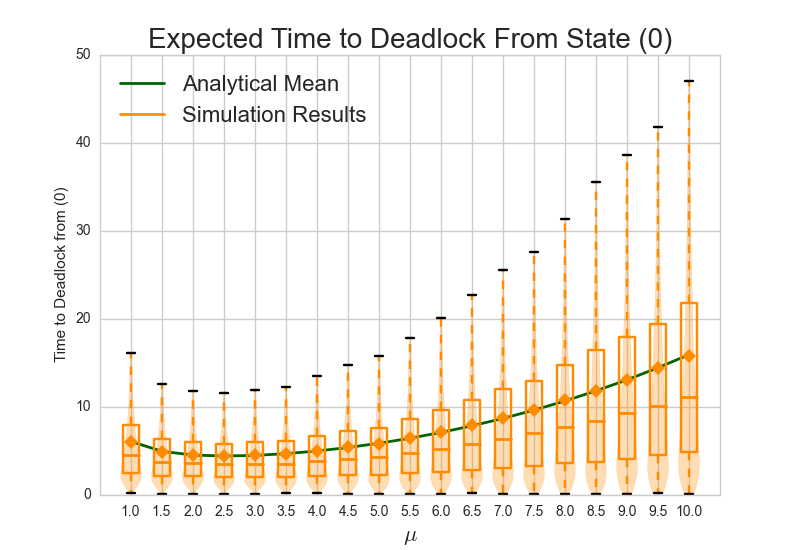
\includegraphics[width=\textwidth]{images/varymu}
  \caption{Varying $\mu$}
  \label{fig:timestodeadlock_mu}
\end{subfigure}
\begin{subfigure}[b]{0.5\textwidth}
  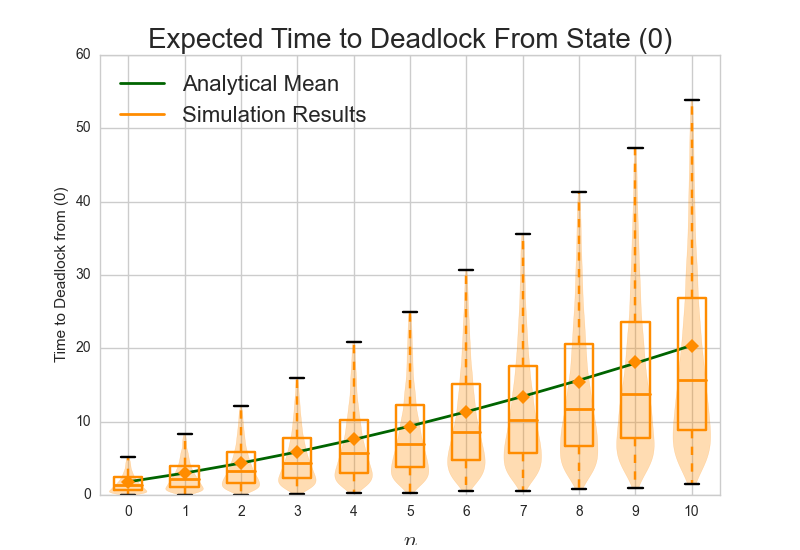
\includegraphics[width=\textwidth]{images/varyn}
  \caption{Varying $n$}
  \label{fig:timestodeadlock_n}
\end{subfigure}
\caption{Analytical \& Simulation Results of Times to Deadlock (10,000 iterations)}
\label{fig:timestodeadlock}
\end{figure}

We get interesting behaviour as the service rate $\mu$ varies, as the service rate contributed towards bothmoving customers from the system and allowing customers to rejoin the queue, causing blockages and deadlock.
This behavious can be interperated as follows:
\begin{itemize}
\item At low service rates below a certain threshold, the arrival rate is relatively large compared to the service rate, and we can assume a saturated system.
At this point services where a customer exits the system does not have much of an effect, as we can assume another arrival immediately.
However services where a customer wishes to rejoin the queue results in a blockage as the system is saturated.
Therefore, increasing the service rate here increases the chance of a blockagße, and so the chance of deadlock.
\item Above this threshold the service rate is large enough that we cannot assume a saturated system, and so services where the customer exits the system does have an affect on the number of customers in the system.
Thus increasing the service rate removes people from the system, and as sush there is less chance of getting blocked and deadlocked.
\end{itemize}

This effect is closely related to the transition rate $r_{11}$, as the rate at which the system enters deadlock from a full queue is $r_{11}\mu$.
Figure~\ref{fig:varymuandr} shows the effect of the transition rate on the behaviour of varying the service rate.

\begin{figure}
  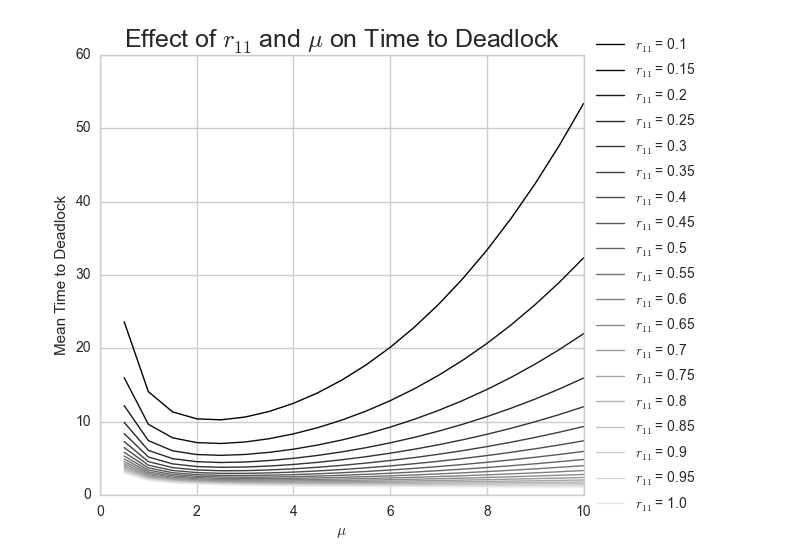
\includegraphics[width=\textwidth]{images/varymur11}
  \caption{The effect of $r_{11}$ and $\mu$ on times to deadlock.}
  \label{fig:varymuandr}
\end{figure}

\subsection{Two Node Network without Self Loops}
Consider the queueing network shown in Figure~\ref{fig:queueingnetwork_2nodes}.
This shows two \(M/M/1\) queues, with \(n_i\) queueing capacity at at each service station and service rates $\mu_i$.
$\Lambda_i$ is the external arrival rates to each service station.
All routing possibilities except self loops are possible, where the routing probability from node $i$ to node $j$ is denoted by $r_{ij}$.

\begin{figure}[H]
  \includestandalone[width=\textwidth]{images/2nodeexample}
  \caption{A two node queueing network.}
  \label{fig:queueingnetwork_2nodes}
\end{figure}

\begin{itemize}
    \item State space:
        \[S = \{(i,j)\in\mathbb{N}^{(n_1+2\times n_2+2)}| 0 \leq i + j \leq n_1 + n_2 + 2
        \}\cup\{(-1, -1)\}\]

        where \(i\) denotes number of individuals:
            \begin{itemize}
                \item In service or waiting at the first node.
                \item Occupying a server but having finished service at the
                    second node waiting to join the first
            \end{itemize}
        where \(j\) denotes number of individuals:
            \begin{itemize}
                \item In service or waiting at the second node.
                \item Occupying a server but having finished service at the
                    first node waiting to join the first
            \end{itemize}
        and the state $(-1)$ denotes the deadlocked state.
\end{itemize}

If we define $\delta = (i_2, j_2) - (i_1, j_1)$ for all $(i_k, j_k) \in S$, then the transitions are given by:

\begin{equation}
  q_{(i_1, j_1),(i_2, j_2)} = \left\{
  \begin{matrix*}[ r ]
    \left. \begin{matrix*}[ r ]
      \Lambda_1 & \text{if } i_1 < n_1 + 1 \\
      0 & \text{otherwise}
    \end{matrix*} \right\} & \text{if } \delta = (1, 0) \\
    \left. \begin{matrix*}[ r ]
      \Lambda_2 & \text{if } j_1 < n_2 + 1 \\
      0 & \text{otherwise}
    \end{matrix*} \right\} & \text{if } \delta = (0, 1) \\
    \left. \begin{matrix*}[ r ]
      (1 = r_{12})\mu_1 & \text{if } j_1 < n_1 + 2 \\
      0 & \text{otherwise}
    \end{matrix*} \right\} & \text{if } \delta = (-1, 0) \\
    \left. \begin{matrix*}[ r ]
      (1 - r_{21})\mu_2 & \text{if } i_1 < n_1 + 2 \\
      0 & \text{otherwise}
    \end{matrix*} \right\} & \text{if } \delta = (0, -1) \\
    \left. \begin{matrix*}[ r ]
      r_{12}\mu_1 & \text{if } j_1 < n_2 + 2 \text{ and } (i_1, j_1) \neq (n_1 + 2, n_2) \\
      0 & \text{otherwise}
    \end{matrix*} \right\} & \text{if } \delta = (-1, 1) \\
    \left. \begin{matrix*}[ r ]
      r_{21}\mu_2 & \text{if } i_1 < n_1 + 2 \text{ and } (i_1, j_1) \neq (n_1, n_2 + 2) \\
      0 & \text{otherwise}
    \end{matrix*} \right\} & \text{if } \delta = (1, -1) \\
    0 & \text{otherwise}
  \end{matrix*} \right.
\end{equation}

\begin{equation}
  q_{(i_1, j_1), (-1)} = \left\{
  \begin{matrix*}[ r ]
    r_{21}\mu_2 & \text{if } (i, j) = (n_1, n_2 + 2) \\
    r_{12}\mu_1 & \text{if } (i, j) = (n_1 + 2, n_2) \\
    0 & \text{otherwise}
  \end{matrix*}
  \right.
\end{equation}

and

\begin{equation}
  q_{-1, s} = 0
\end{equation}

For $n_1 = 1$ and $n_2 = 2$, the resulting Markov chain is shown in Figure~\ref{fig:2nodeMC}.

\begin{figure}[H]
    \includestandalone[width=\textwidth]{images/markov_chain}
    \caption{Markov chain of the two node system with $n_1=1$ and $n_2=2$.}
    \label{fig:2nodeMC}
\end{figure}

Figure~\ref{fig:timestodeadlock2} shows the effect of varying the parameters of the above Markov model.
Only parameters for one node are shown, as the other node's parameters will have the same affect.
We can see that we get similar behaviour as the 1 node network.

\begin{figure}[H]
\begin{subfigure}[b]{0.5\textwidth}
  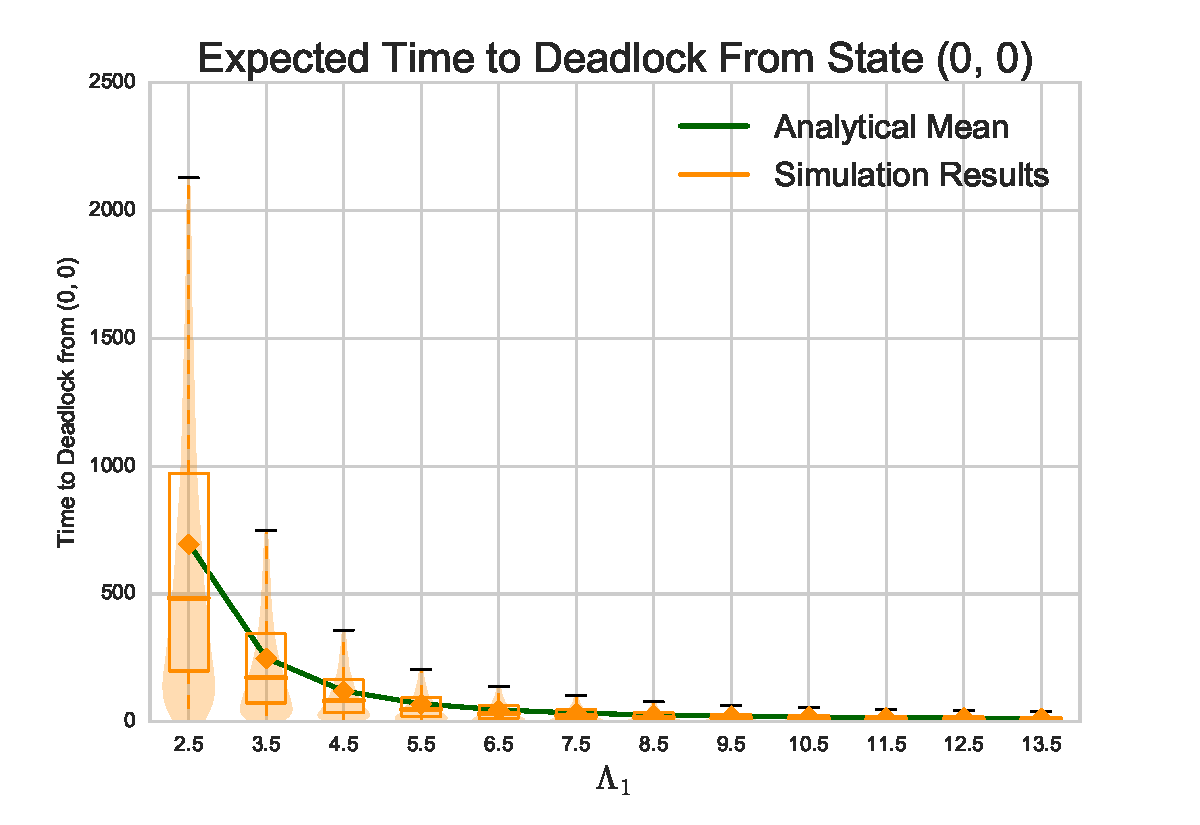
\includegraphics[width=\textwidth]{images/varyL1}
  \caption{Varying $\Lambda_1$}
  \label{fig:timestodeadlock2_L1}
\end{subfigure}
\begin{subfigure}[b]{0.5\textwidth}
  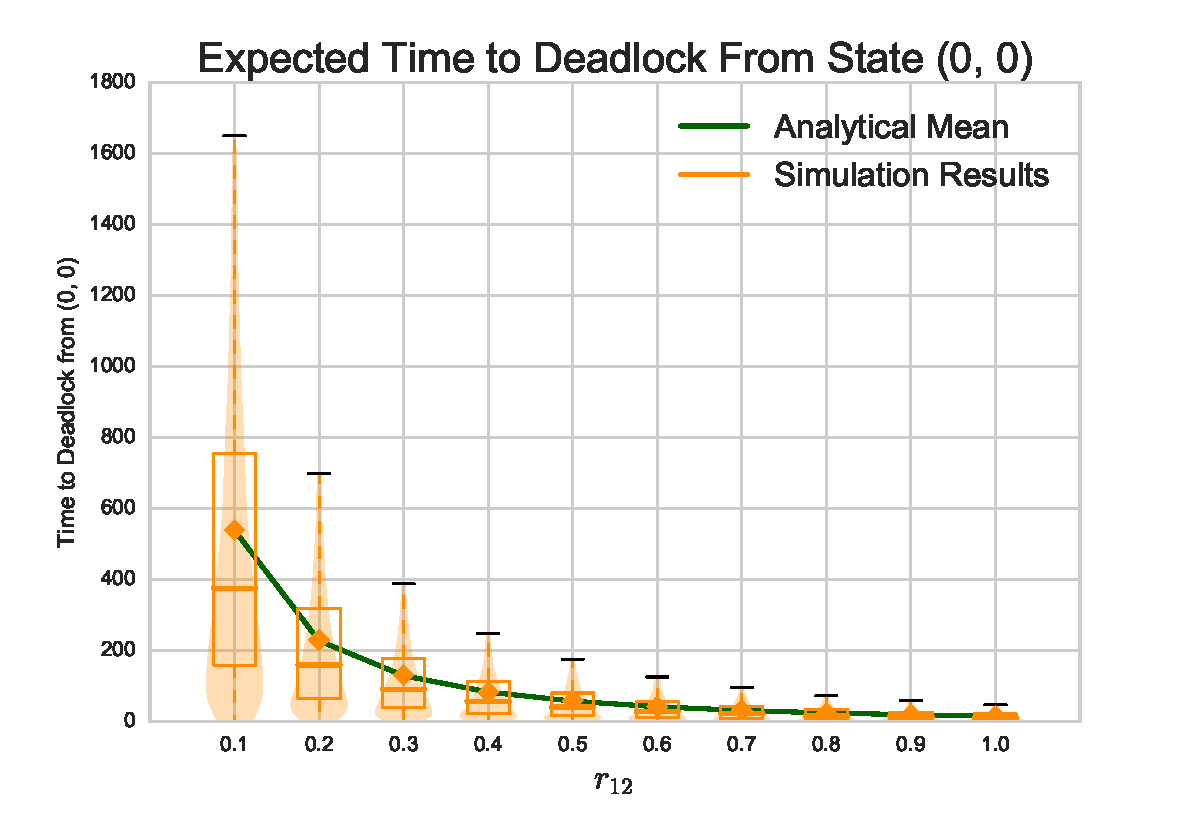
\includegraphics[width=\textwidth]{images/varyr12}
  \caption{Varying $r_{12}$}
  \label{fig:timestodeadlock2_r12}
\end{subfigure}
\begin{subfigure}[b]{0.5\textwidth}
  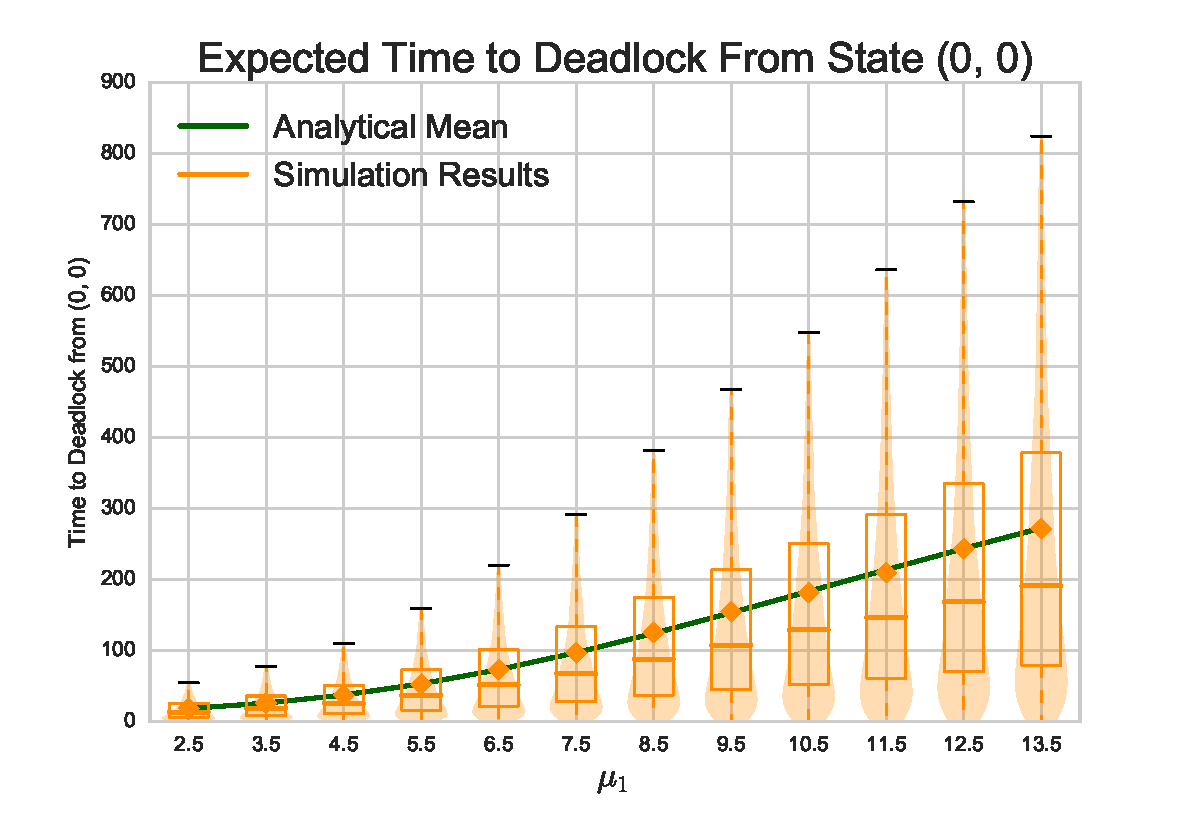
\includegraphics[width=\textwidth]{images/varymu1}
  \caption{Varying $\mu_1$}
  \label{fig:timestodeadlock2_mu1}
\end{subfigure}
\begin{subfigure}[b]{0.5\textwidth}
  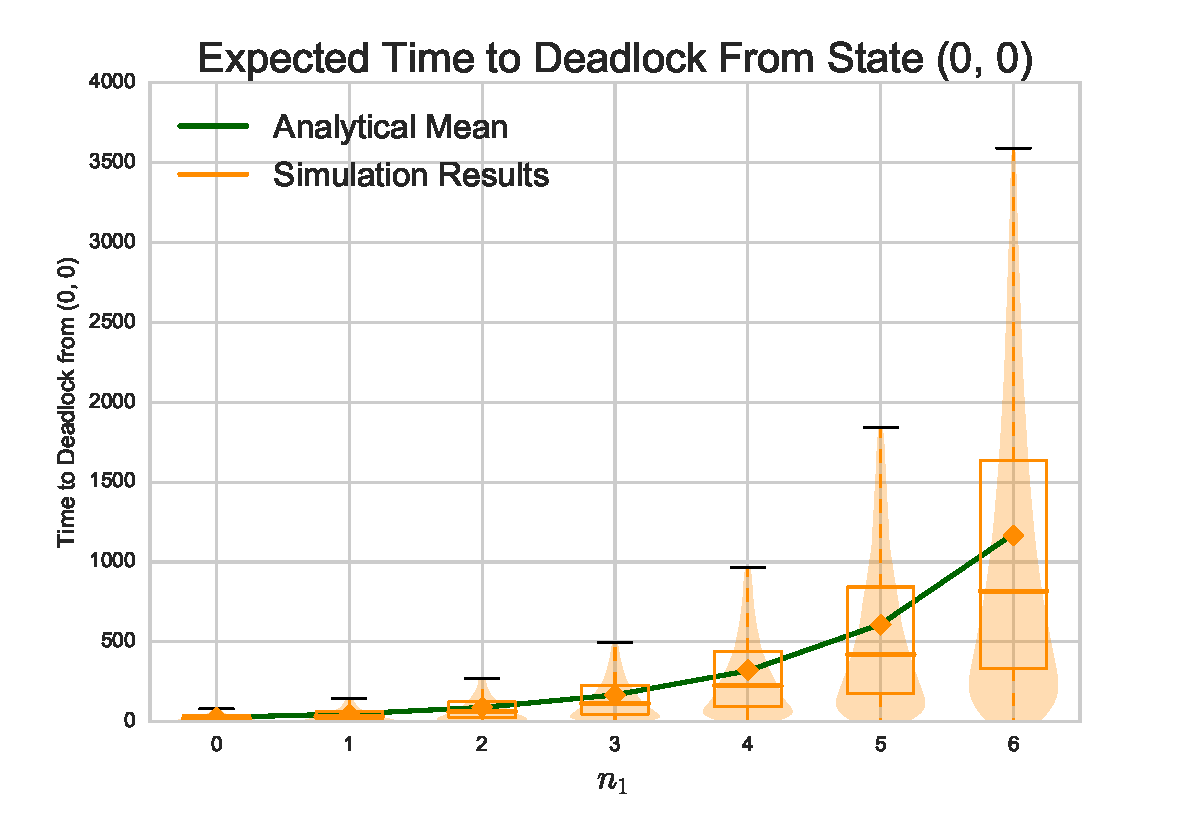
\includegraphics[width=\textwidth]{images/varyn1}
  \caption{Varying $n_1$}
  \label{fig:timestodeadlock2_n1}
\end{subfigure}
\caption{Analytical \& Simulation Results of Times to Deadlock (10,000 iterations)}
\label{fig:timestodeadlock2}
\end{figure}


\section{Resolving Deadlock}
Once the system falls into a deadlocked state for the first time, that is the first transient deadlocked state since the last resolution, the simulated needs to automatically resolve the deadlock and allow services to resume again.
This is not necassarily as simple as moving a blocked customer to his next node, as we need to conserve the numbers of customers at each service station.
Closer inspection of the state digraph is required in order to find a way to resolve deadlock whilst conserving this property.

At deadlock, the service stations can be classified into the following three mutually exclusive categories:
\begin{itemize}
    \item Nodes that are not deadlocked: These are nodes that do not contain any blocked individuals.
    \item Causation nodes, nodes causing deadlock: These are nodes where every server is occupied by a blocked individual, and there is at least one blocked individual waiting to enter that node who is directly or indirectly being blocked by an individual in this node.
    \item Affected nodes, nodes affected by deadlock: These are nodes containing at least one blocked individual who is directly or indirectly being blocked by an individual at a node that is causing deadlock, but is not classified as causing deadlock itself.
\end{itemize}

At the first instance of deadlock, there will only be one knot in $D(t)$.
Let us denote the knot as $K$.
The vertices of $K$ correspond to servers.
As there is no sink node, all vertices of $K$ have an out-edge, and so all vertices in $K$ contain a blocked individual.
Therefore, there are no vertices in $K$ belonging to nodes that are not deadlocked.
All vertices of $K$ correspond to servers of causation nodes, and a causation node has all its servers belonging to $K$.
An affected node has servers belonging to the same weakly connected component as $K$, but does ot have servers in $K$.

When choosing which customer to move in order to resolve deadlock, we must be careful to conserve the number of customers at each service station.
Causation nodes have full queues, and a customer may only be moved into a full queue if this causes another customer to simultaneously move from this node.
Another complication arises due to the blocking mechanism used, in which those customers who have been blocked longer must be moved first.
This property may have to be broken in order to ensure the conservation property is not.
Assume that we have weighted the edges of the digraph with the time that they were created. % If this works then I'll include this in the write up of how state digraph is formed

The following algorithm is proposed in order to resolve deadlock:

\begin{algorithm}[H]
    \DontPrintSemicolon
    Find the knot $K$ in $D(t)$\;
    Find the cycle $C \in K$ whose average edge weight is minimum\;
    Start at $V_0$\;
    \For{$V_i$ in $C$}{
    Move the individual who is waiting to get to $V_{i+1}$\;}
    Redraw $D(t)$\;
\end{algorithm}



\bibliographystyle{plain}
\bibliography{refs}





\end{document}
